
%% main.tex (V1, 2020/05/04)
%% template for the group reports for 4SC070 Learning Control based on the template for IEEE journal papers (V1.4b, 2015/08/26 by Michael Shell)

%%
%% This is a skeleton file demonstrating the use of IEEEtran.cls
%% (requires IEEEtran.cls version 1.8b or later) with an IEEE
%% journal paper.



\documentclass[journal]{IEEEtran}
%
% If IEEEtran.cls has not been installed into the LaTeX system files,
% manually specify the path to it like:
% \documentclass[journal]{../sty/IEEEtran}


\usepackage{graphicx}      % include this line if your document contains figures
\usepackage{cite}        
\usepackage{siunitx}
\usepackage{amssymb}
\usepackage{amsmath}
\usepackage{fancyhdr}
\usepackage{caption} % Allows for fancy caption options
\usepackage{subcaption} % Allows for subfigures
\usepackage[framed,numbered,autolinebreaks,useliterate]{mcode}

\usepackage{bbold}
\usepackage{hyperref}

\usepackage[english]{babel}
\addto\extrasenglish{
  \def\subsubsectionautorefname{Section}
  \def\subsectionautorefname{Section}
  \def\sectionautorefname{Section}
}


\begin{document}
%
% paper title
% Titles are generally capitalized except for words such as a, an, and, as,
% at, but, by, for, in, nor, of, on, or, the, to and up, which are usually
% not capitalized unless they are the first or last word of the title.
% Linebreaks \\ can be used within to get better formatting as desired.
% Do not put math or special symbols in the title.
\title{Matched Basis Function Repetitive Control for Multi-Frequency Disturbances}
%
%
% author names 
% note positions of commas and nonbreaking spaces ( ~ ) LaTeX will not break
% a structure at a ~ so this keeps an author's name from being broken across
% two lines.


\author{Max~Jans,
        Mustafa~Doğan,
        Olaf~Wijdeven}
% 



% The paper headers
\markboth{4SC070 Learning Control}%
{Report Template}
% The only time the second header will appear is for the odd numbered pages
% after the title page when using the twoside option.

% make the title area
\maketitle

% As a general rule, do not put math, special symbols or citations
% in the abstract or keywords.
\begin{abstract}
%The abstract goes here. Guideline: five sentences, describing the background, the aim, the method, the results and the conclusion. 
Many industrial systems experience repetitive disturbances consisting of multiple unrelated frequencies, making traditional repetitive control approaches ineffective due to slow convergence and high complexity. The aim of this research is to develop a robust matched basis function repetitive control method capable of individually suppressing multi frequency disturbances without negatively affecting other system frequencies. Both simplified (using direct projection) and non-simplified (using iterative projection updates) approaches were evaluated through simulations and experimental validation using an Arizona printer setup, with disturbances comprising distinct periodic signals. Results demonstrated significant performance improvements. The simplified approach effectively reduced disturbances and was straightforward to implement. The non-simplified approach achieved faster convergence rates while still effectively reducing disturbances. The findings emphasize matched basis function repetitive control's potential for industrial systems.
\end{abstract}



\section{Introduction}
% The very first letter is a 2 line initial drop letter followed
% by the rest of the first word in caps.
% 
% form to use if the first word consists of a single letter:
% \IEEEPARstart{A}{demo} file is ....
% 
% 
% Here we have the typical use of a "T" for an initial drop letter
% and "HIS" in caps to complete the first word.
\IEEEPARstart{L}{earning} control is an emerging subfield in the greater scope of control engineering. The aim of applying learning control to a system is to increase the performance beyond that which is possible using standard feedback controllers. This is achieved by "beating" causality through the use of knowledge about previous error signals or specifics about disturbances. During the course Learning Control (4SC070) techniques such as Iterative Learning Control (ILC) and Repetitive Control (RC), and some of their sub-categories, were discussed.

In industrial settings, many systems perform repetitive tasks continuously such as, wide-format industrial printing \cite{bevers_research_nodate}, hard drive servo control \cite{noauthor_iterative_nodate} and others. This continuous operation lends itself well to the application of Repetitive control. However, for many complex systems the disturbance signal is comprised of many different frequencies. They can often be related back to a smaller number of primary frequencies. In the case where multiple unrelated frequencies are present, their Least Common Multiple (LCM) may be very large or non-existent. This has the main downside that the periodicity of the disturbance is then also non-existent or very large.

Applying traditional RC to such a system with a large LCM will show very slow performance improvements \cite{luo_repetitive_2016}. To counteract this problem alternative RC structures have been proposed to deal with these types of disturbances. One of these is Matched Basis Function Repetitive Control (MBFRC) \cite{nagashima_analysis_2004}. MBFRC targets individual frequencies independently without interfering with other frequencies. This allows for a modular and scalable RC structure.

The goal of this research is to develop a robust repetitive controller to suppress multiple unrelated periodic disturbances acting on the Arizona printer \cite{Challenge_description}.

In \autoref{sec:Prob_Form} the specifics of the problem that was tackled with this research project are described. \autoref{sec:Approach} shows the control approach that was taken while \autoref{sec:Exp_Res} lays out the results of applying said controller to the printer. Finally in \autoref{sec:Conclusion} the solution to the problem will be evaluated using the information from the previous chapters.
%file is intended as a demo/template for the group reports for the course 4SC070 Learning Control. It is based on the template for IEEE journal papers using
% IEEEtran.cls version 1.8b and later. It is strongly recommended to use the sections mentioned in this template, but feel free to add any sections that you think are relevant. For inspiration on writing in a paper format, see \url{http://toomen.eu/publications.html#journal}.
% % You must have at least 2 lines in the paragraph with the drop letter
% % (should never be an issue)

% During the course, each group will write a report using this template. The report discusses the challenge, and your ideas for a learning algorithm that enables small contouring errors with limited actuator inputs.

% In the introduction, you introduce the problem. Describe the context, the problem, the approach/solution and the structure of this document. Why should the reader read this work? For the challenge report, add some references to existing approaches/ideas in literature.

\section{Problem formulation}\label{sec:Prob_Form}
In the continuous feed printer from Canon Production Printers there exist numerous periodic disturbances coming from different parts such as rollers or the print belt \cite{Challenge_Presentation}. These disturbances need to be attenuated in order to increase printing quality or printing speed. However, since no continuous feed printer was available for this research project an Arizona printer from Canon Production Printers has been used to emulate a similar scenario as in the continuous feed printer. This is achieved by applying a ramp reference in the y-direction of the printer that goes back and forth continuously with a period time of 10 seconds \autoref{fig:yref}. In addition to this a disturbance signal with two distinct period times of 5 and 6 seconds is added to the input of the printer. The power spectrum of this disturbance can be seen in \autoref{fig: PSD_disturbance_real} which shows that there are a lot of single frequency spikes in the error spectrum of the system coming from these frequencies.


The objective for this research project is to find a novel design procedure for robustly stable (simplified) MBFRC to attenuate these frequencies while adhering to a number of requirements:
\begin{enumerate}
    \item[R1] The RC must obtain high tracking performance.
    \item[R2] The RC must be easy to implement, that is, a one-step design procedure is preferred, and the resulting controller order is not extremely high.
    \item[R3] Preferably, the parameters of the RC controller must be easy to adapt in real-time.
    \item[R4] The RC must be robust to model uncertainties, while still effective in suppressing above-bandwidth disturbances.
    \item[R5] The RC must have fast convergence.
\end{enumerate}



\section{Approach}
\label{sec:Approach}
In this chapter we will elaborate on in total three different approaches to reach the requirements stated in \autoref{sec:Prob_Form} as well as stability analysis for MBFRC. The theoretical background for these three approaches will be shown. We will also elaborate on the differences between the methods. Simulation results for the approaches will also be examined to see the effectiveness of each method, in terms of convergence speed and error reduction. The basic implementation of adding an MBFRC controller can be seen in \autoref{fig:BlkDiaRC}.

\begin{figure}[!t]
    \centering
    \includegraphics[width=0.8\linewidth]{figures/simple_MBFRC/MBFRC_schematic.png}
    \caption{Block diagram showing the control schematic when using MBFRC}
    \label{fig:BlkDiaRC}
\end{figure}
\subsection{Simplified MBFRC}\label{ssec: SimplifiedMBFRC}
MBFRC uses periodic sinusoidal basis functions in order to attenuate periodic disturbances. It is able to attenuate singular frequencies whereas traditional RC attenuates a disturbance frequency and all of it's higher harmonics. 

\subsubsection{Theoretical background}\label{sssec: SimplifiedMBFRC_Theory}
The first step for applying MBFRC is the projection step. This makes a projection from the error \(e_k\) to an intermediate vector \(\vec\beta_k\). For simplified MBFRC this is done as follows
\begin{subequations}\label{eq: ProjectionSimplifiedMBFRC}
\begin{equation}
\vec\beta_k = H_k^\top \vec e_k
    \end{equation}
    \begin{equation}
        H_k^\top = \begin{bmatrix}
            \cos(\omega_1 k T_s)  &\cdots & 0\\
            \sin(\omega_1 k T_s)&
        \cdots &0\\
        \vdots&\ddots&\vdots\\
        0&\cdots&\cos(\omega_N k T_s)\\
        0&\cdots &\sin(\omega_N k T_s)
        \end{bmatrix}
        \end{equation}
        \begin{equation}
        \vec e_k = \mathbb{1}_N\cdot e_k
\end{equation}
\end{subequations}
where, $\vec\beta_k\in\mathbb{R}^{2N}, \:H_k \in\mathbb{R}^{N\times 2N},\:\vec e_k \in\mathbb{R}^N\:e_k\in\mathbb{R}$ and \(\mathbb{1}_N\) is a vector of ones of length N, where N is the number of attenuated frequencies. Then the second step is to apply the RC control action which translates the basis function coefficients \(\vec\beta_k\) to the RC action vector known as \(\vec\alpha_k\). This is done as follows
\begin{equation}
    \begin{aligned}
        \vec\alpha_k = \vec\alpha_{k-1}+\phi\vec\beta_k\\
    \end{aligned}
\end{equation}
where, $\vec\alpha_k\in\mathbb{R}^{2N} \:\text{and}\:\phi\in\mathbb{R}^{2N\times 2N}$ and \(\phi\) is the repetitive control gain and is either a scalar or a matrix shaped as follows
\begin{equation}
    \begin{aligned}
        \phi = \begin{bmatrix}
            \phi_1&0&\cdots & 0 & 0\\
            0 & \phi_1 &\cdots&0&0\\
            \vdots & \vdots & \ddots & \vdots & \vdots\\
            0&0&\cdots&\phi_N&0\\
            0 & 0 & \cdots &0 & \phi_N
        \end{bmatrix}
    \end{aligned}
\end{equation}
The RC action \(\vec\alpha_k\) is then used in the step to get the command input which is the output of the MBFRC controller. This is done using the formula
\begin{subequations}
    
\begin{equation}
        \vec{RC_k} = G_k\vec\alpha_k
\end{equation}
\begin{equation}
        G_k^\top = \begin{bmatrix}
            \frac{1}{r_1}\cos(\omega_1 k T_s-\tau_1)  &\cdots & 0\\
            \frac{1}{r_1}\sin(\omega_1 k T_s-\tau_1)&
        \cdots &0\\
        \vdots&\ddots&\vdots\\
        0&\cdots&\frac{1}{r_N}\cos(\omega_N k T_s-\tau_N)\\
        0&\cdots &\frac{1}{r_N}\sin(\omega_N k T_s-\tau_N)
        \end{bmatrix}
\end{equation}
\end{subequations}
where, $\vec{RC_k}\in\mathbb{R}^N\: \text{and}\:G_k\in\mathbb{R}^{N\times 2N}$ If multiple frequencies are being attenuated this \(\vec{RC}_k\) needs to be summed such that \(RC_k = \vec{RC}_k^\top\mathbb{1}_N\). This $RC_k$ is what is passed to the controller of the system. These past steps can also be seen in a block diagram in \autoref{fig:BlkDiaSimp} for the scalar case where only one frequency is attenuated.

\begin{figure}[!t]
    \centering
    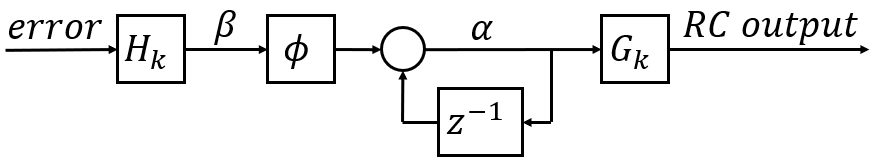
\includegraphics[width=0.9\linewidth]{figures/simple_MBFRC/simple_MBFRC_2.png}
    \caption{Block diagram showing the internals of the simplified MBFRC}
    \label{fig:BlkDiaSimp}
\end{figure}
\subsubsection{Simulation}\label{sssec: SimplifiedMBFRC_Simulation}
Simulations in Simulink \cite{Simulink_website} are performed to test performance and stability of the MBFRC algorithm. This has been done while iteratively increasing the number of attenuated frequencies. The PSD is taken over a period of 30 seconds to ensure that all frequencies from the 5 second and 6 second disturbance can complete full periods in the mentioned time window of 30 seconds. This means that a full disturbance signal is needed in which the MBFRC has converged to see the performance, resulting in at least 2 full disturbance periods being needed. The reference for the simulations for the (non) simplified MBFRC is turned off. This is done as it does not interfere with stability and would make the disturbance rejection more difficult to see in the PSD plots, as the power at the reference frequencies is much greater. The best result in terms of error reduction can be seen in \autoref{fig:sim48simp} located in \autoref{app:SimSim}. The simulation is performed while attenuating all 47 frequencies in the disturbance as well as DC for 4 times the disturbance signal of 30 seconds. The values in the $\phi$ matrix for this simulation were set to $0.0001$ for all 48 frequencies. The image shows that the error reduces quickly and even during the first LCM of the disturbances which would not be possible with traditional RC. However, because this is a simulation and all disturbances are being rejected and no additional noise is present the L2 norm of the error reduces indefinitely or until the smallest possible value in  MATLAB is reached. This does not happen when working with a real system as zero error can never be achieved due to multiple causes like sensor accuracy and extra stochastic disturbances. For more simulations see \autoref{app:SimSim}.


\subsection{Non-simplified MBFRC}\label{ssec: NonSimplifiedMBFRC}
Non-simplified MBFRC is very similar in its workings to simplified MBFRC, there are some crucial differences which increase the complexity but should also increase its performance.
\subsubsection{Theoretical background}\label{sssec: NonSimplifiedMBFRC_Theory}
The main difference between simplified and non-simplified MBFRC is the projection step. Previously the projection was defined as in \autoref{eq: ProjectionSimplifiedMBFRC}. The projection step for the non-simplified MBFRC differs in the fact that $\vec\beta$ is not determined by a multiplication, but rather with an iterative process. The definition for $\vec\beta$ will become 
\begin{equation}
\begin{aligned}\label{eq: ProjectionNonSimplifiedMBFRC}
    \vec\beta_k=\vec\beta_{k-1}+aH_k^\top (e_k-H_k\vec\beta_{k-1}).
\end{aligned}
\end{equation}
Where,  $a\in\mathbb{R}^{2N}$ and, $H_k$ and $e_k$ are again the projection matrix and error signal as defined in \autoref{sssec: SimplifiedMBFRC_Theory}. This does complicate the model, and therefore might not be a perfect fit for systems where computation power is very limited. In contrast to the simplified MBFRC, this algorithm uses an integrator to determine the $\vec\beta_k$, which can also be seen in \autoref{fig: nonSimpleMBFRC_blocks}, this increases the storage needed in the system. 
\begin{figure}[!t]
    \centering
    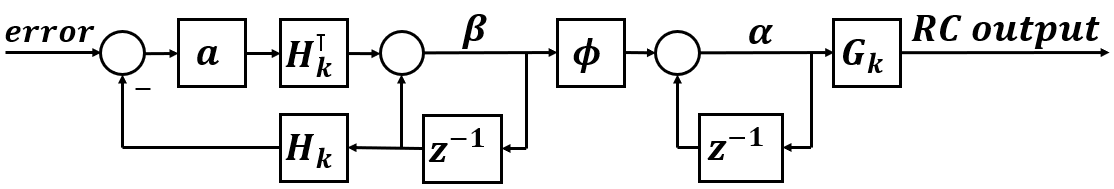
\includegraphics[width=1\linewidth]{figures/nonSimple_RC_MBFRC/non_simple_MBFRC_2.png}
    \caption{Block diagram of the non-simplified MBFRC algorithm}
    \label{fig: nonSimpleMBFRC_blocks}
\end{figure}

The biggest difference between simplified and non-simplified MBFRC, according to \cite{zwaans_frequency_nodate}, is that the projection and repetitive control action are separated in the non-simplified algorithm. This separation contributes that the output basis function coefficients $\vec\beta_k$ can be used to make a fit on the error for a certain period of time, before applying these changes on the repetitive control gains $\alpha$. This makes the non-simplified algorithm more robust to the disturbance changing over time.   

\subsubsection{Simulation}\label{sssec: NonSimplifiedMBFRC_Simulation}
To test the performance of the non-simplified MBFRC algorithm, simulations are done in Simulink. As in \autoref{sssec: SimplifiedMBFRC_Simulation} only the best performing simulation will be discussed here and some more results are elaborated on in \autoref{app:nonSimSim}. \autoref{fig:nonSimpSim48} shows the results for a simulation where all 47 disturbance frequencies are attenuated in addition to DC. The $\phi$ and $a$ values are 0.0002 and 0.001 for all frequencies respectively. The simulation is performed for 4 periods to allow for easy comparison to the simplified MBFRC. When comparing \autoref{fig:sim48simp} to \autoref{fig:nonSimpSim48} it shows that the error reduces much faster and after four periods the L2 norm is a factor \(10^6\) times smaller. Although this result should not be taken at face value as this is a simulation with no outside disturbances, the faster convergence should also happen in real life. More simulation results can be seen in \autoref{app:nonSimSim}



\subsection{Cascaded RC with MBFRC}\label{ssec:cascadedRC}
Applying the reference signal to the system introduces a new disturbance at $0.1 Hz$ with higher harmonics up to the Nyquist frequency of $500 Hz$. This would be extremely difficult to attenuate using MBFRC as it would increase the matrix sizes and would require $\phi$ to become even lower increasing convergence time. The increase in matrix sizes could also increase computational load too much. A solution we propose is to use traditional RC in a cascaded form with MBFRC. This allows the MBFRC to attenuate the disturbance frequencies such that the error can already decrease during the first reference period. And the traditional RC controller can attenuate the base frequency and its harmonics of the reference signal.



\subsubsection{Theoretical background}
Performing multi-period RC with multiple traditional RC controllers is well documented as in for example \cite{SequentialRC}. However, doing this same cascaded design using RC and MBFRC is not well documented in literature. A block diagram of the used cascaded structure can be seen in \autoref{fig:BLKcascade}.

\begin{figure}
    \centering
    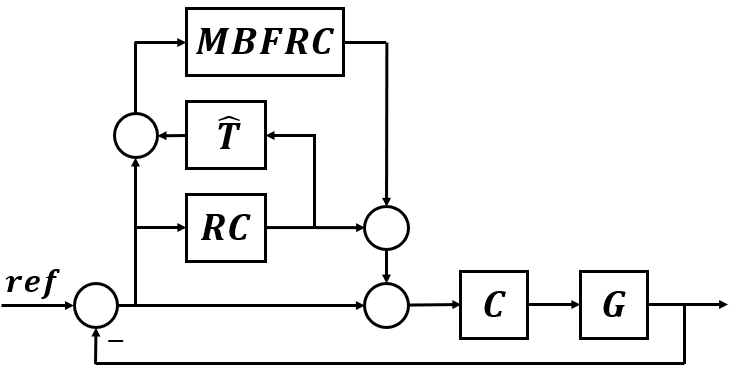
\includegraphics[width=0.8\linewidth]{figures/simple_RC_MBFRC/MBFRC_RC_2.png}
    \caption{Block diagram showing the cascaded form using RC and MBFRC}
    \label{fig:BLKcascade}
\end{figure}

The used cascade structure is very similar to the structure used in traditional sequential RC, the only difference being that the second RC controller is exchanged with an MBFRC controller. The sequential loop closing works through making an equivalent plant $T_2^{eq}$,
\begin{equation}
    T_2^{eq} = \frac{1+\hat TR_1}{1+TR_1}T
\end{equation}
where $\hat T$ is a parametrized model of the closed loop dynamics and $T$ is an frf measurement of the closed loop. The output of $T_2^{eq}$ is taken as the error for the second RC controller. The design of this $T_2^{eq}$ is such that the output of it is as close as possible to the remaining error after the RC signal from the first controller is applied to the system. If $\hat T=T$ the two RC controllers are completely decoupled meaning that the second RC controller can be synthesized based only on T. 
Replacing the second RC controller with MBFRC only changes the stability guarantees of the implementation. No new guarantees have been found for this implementation and as such a conservative RC controller was implemented. In addition to this, conservative values for MBFRC were chosen.
\subsubsection{Simulation}\label{sssec:CascadedSim}
For the simulations with the cascaded design, the reference has been turned on as the RC controller is designed to attenuate the reference signal. As before, multiple simulations have been performed for this use case but only the best result will be discussed here. The best results were achieved when using non-simplified MBFRC with $a = 0.001$ and $\phi = 0.0001$. For the RC controller the complementary sensitivity was inverted using ZPETC \cite{Tomizuka_1987} and a Q filter is designed by using a 12-th order $\operatorname{fir1}$ filter and putting the normalized frequency at $0.1Hz$. This results in a simulation as seen in \autoref{fig:cascNonSimp} located in \autoref{app:simCasc} where it shows that after one reference signal, the reference gets reduced significantly by the RC controller. The L2 norm of the error is however much greater than before and does not reduce indefinitely anymore due to the high frequency harmonics of the reference. They are not attenuated by the RC controller because they are above the bandwidth of the Q filter.

\subsection{Stability analysis}
To be able to guarantee stability of a system with MBFRC implemented, the eigenvalues of the sensitivity function can be checked for unstable poles \cite{zwaans_frequency_nodate}. However, this can only guarantee stability in case the parameters such as the values of $a$ and $\phi$ are already known. This property can be used to manually tune these parameters to their maximum values before instability occurs. Manually tuning these parameters can however become very time intensive when more and more frequencies are added to be attenuated. While \cite{shi_small_2014} states that the values for $\phi$ should simply be 'low enough', this statement does help for a first try but in the case there are more than a few different frequencies that need to be attenuated, manual tuning becomes increasingly more difficult and cumbersome. Increasing the values of $\phi$ and $a$ increases the convergence rate, meaning the desired performance is reached faster. Therefore the main question of stability becomes: how high can the parameters $a$ and $\phi$ be, before the system becomes unstable?

One of the possible ways to determine these values is via an optimization algorithm. This algorithm needs to have the sum or any combination of the parameters as its cost function. The only constraint on the stability is that the eigenvalues of the sensitivity function should all be stable, which for discrete systems comes down to that each eigenvalue should be within the unit circle in the z-plane. Using these two criteria, an optimization problem for simplified MBFRC, where the only parameter is $\phi$, can be defined as
\begin{subequations}
\begin{align}\label{eq:OptimizationStability}
    \min_{\phi} \quad & -\sum_{i=1}^{N}(\phi_i )\\
    s.t. \quad & |\lambda(S_{MBFRC}(\phi))|<1.
\end{align}
\end{subequations}
In \autoref{eq:OptimizationStability}, $S_{\text{MBFRC}}$ is defined as the sensitivity of the control loop including an estimation of the MBFRC $M(\phi)$ as in \cite{zwaans_frequency_nodate}
\begin{align}
    S_{MBFRC}=\frac{1}{1+GC(I+M(\phi))}.
\end{align}
Depending on the solver, the cost function and/or constraint could need to be rearranged to fit the solver limitations. This optimization problem can now be solved to give the $\phi$'s that have a maximum value while still stabilizing the system. 

However, the resulting values of $\phi$ stabilize the parameterized model of the system rather than the real system, which will always be slightly different to the models. This means that the optimization problem might need the possibility to add robustness margins on the constraints. For this, the nyquist plot of the open loop system ($CG$) needs to be checked for stability, however, this likely comes back to manual tuning, as it is very complex to implement this criteria in the optimization problem. For now, it is recommended to simply take a 'safety factor' on the optimal $\phi$'s from the optimization and check the nyquist plot manually, tuning where necessary for stability. This is a field where more research is still needed, and thus the stability is not yet translated to a robust setting.

A different approach to investigating the stability of the system was also taken. This second approach entailed dividing the frequency grid into 3 sections, below the controller bandwidth (BW), around the BW and above the BW. For each of these sections 3 frequencies where chosen and then MBFRC is used to attenuate these 3 frequencies. For each section individually the system is simulated over and over while increasing one of the tuning parameters. Then if the simulation became unstable this value was saved. In \autoref{tab:stabilitySimp} the results can be seen for simplified MBFRC this shows there is little difference between below and around the BW while there is a factor 1.6 difference between around BW and above the BW. \autoref{tab:stabilityNonSimp} shows that for $\phi$ only above the BW is different to the others by a factor 2.6. However, looking at $a$ shows that this difference becomes much larger, it is now 866 times larger.

\begin{table}[]
\centering
\caption{Table showing at which values the simulation became unstable for simplified MBFRC}
\label{tab:stabilitySimp}
\begin{tabular}{|l|l|l|l|}
\hline
       & Below BW & Around BW & Above BW \\ \hline
$\phi$ & 0.023     & 0.022      & 0.036    \\ \hline
\end{tabular}
\end{table}

\begin{table}[]
\centering'
\caption{Table showing at which values the simulation became unstable for non-simplified MBFRC}
\label{tab:stabilityNonSimp}
\begin{tabular}{|l|l|l|l|}
\hline
       & Below BW & Around BW & Above BW \\ \hline
$\phi$ & 0.01     & 0.01      & 0.026    \\ \hline
$a$    & 0.0006   & 0.0006    & 0.52     \\ \hline
\end{tabular}
\end{table}
\section{Experimental results}\label{sec:Exp_Res}
In this section the aforementioned methods and algorithms are applied to an Arizona printer \cite{Challenge_description} that was available for measurements. Both a feedback and feedforward controller were already implemented on the system, this controller will not be changed, only additions will be made in the form of a repetitive controller. Constant values of $\phi_i=0.0001$ and where applicable, $a=0.001$, were used. This chapter will go into the experiments that were performed using this system, discussing the results and challenges.

\subsection{Simplified MBFRC}
The simplified MBFRC was first implemented taking only a single frequency of $\frac{1}{6}Hz$ to attenuate, with the resulting Power Spectral Density (PSD) and Cumulative Amplitude Spectrum (CAS), as can be seen in \autoref{fig:FB_comp_simp_MBFRC_1_6s}, in comparison to only using the aforementioned feedback and feedforward controllers.
\begin{figure}
    \centering
    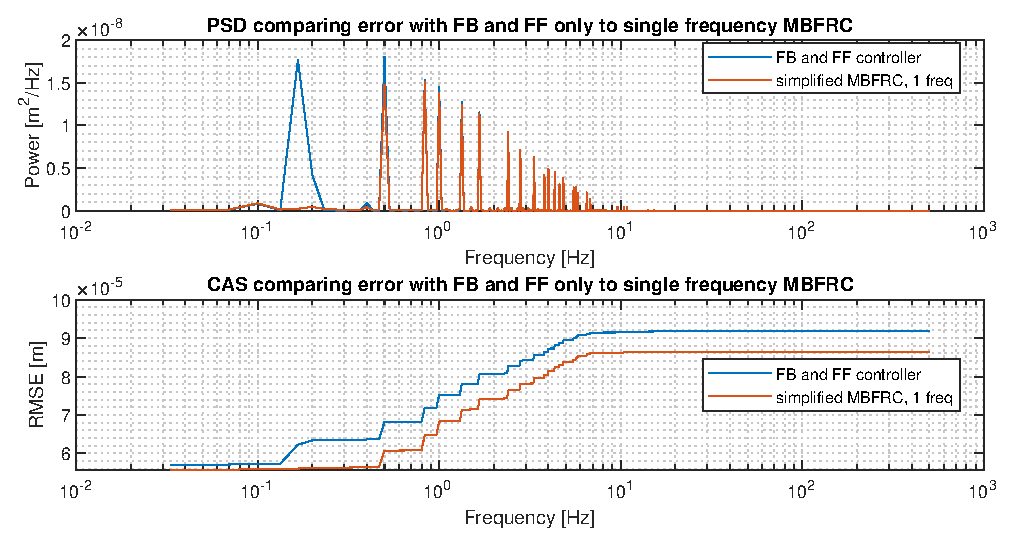
\includegraphics[width=0.9\linewidth]{figures/simple_MBFRC/comp_MBFRC_FB_PSD_CAS_2.eps}
    \caption{CPS and CAS using simplified MBFRC with a single frequency of $\frac{1}{6}$Hz}
    \label{fig:FB_comp_simp_MBFRC_1_6s}
\end{figure}
After this experiment concluded that the designed MBFRC works as expected, more frequencies were added to attenuate. With the PSD of the (non-setpoint) disturbances already known, all the frequencies that had power were added to be attenuated ($47$ frequencies total), a 'basis function' of $0$ was also added to that list, eventually also adding a few of the first harmonics of the setpoint, coming to a total of 51 frequencies. The gradual decrease of total error can easily be seen as more frequencies are added in \autoref{fig:simp_MBFRC_multiple}, totaling to a decrease of slightly more than a factor 5, as can be seen from the CAS.
\begin{figure}
    \centering
    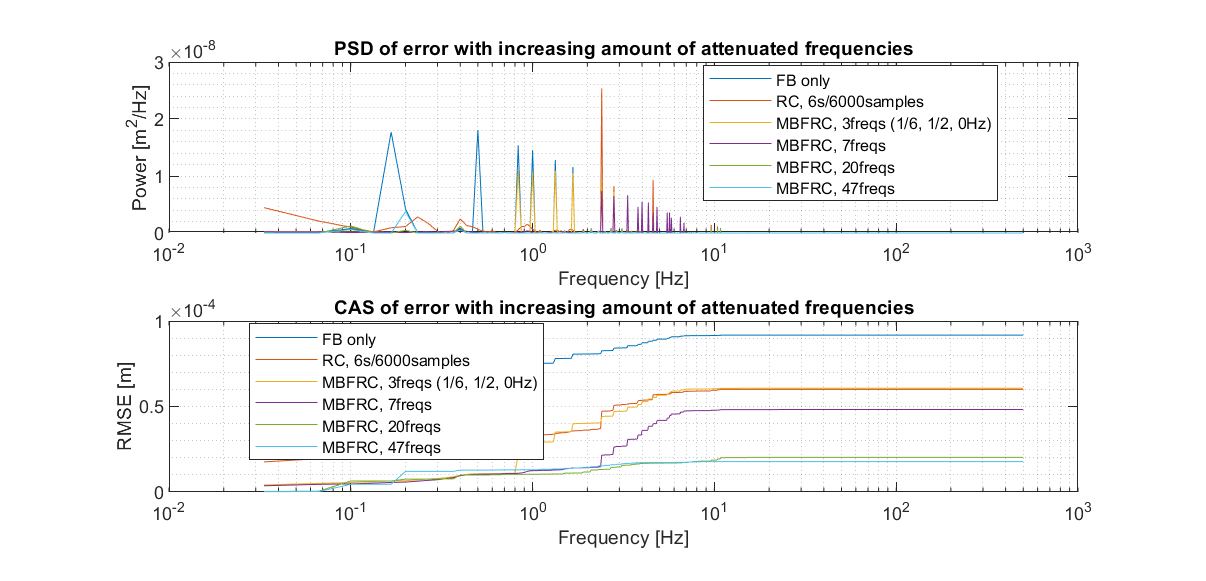
\includegraphics[width=1\linewidth]{figures/simple_MBFRC/comp_moreFreqs_PSD_CAS_2.eps}
    \caption{CPS and CAS using simplified MBFRC with an increasing amount of frequencies}
    \label{fig:simp_MBFRC_multiple}
\end{figure}
This proves that simplified MBFRC alone has a huge effect on the systems performance, even after just a few setpoint cycles.

\subsection{Non-simplified MBFRC}
Using the non-simplified MBFRC, the performance of the system should become even better. To be more precise, the convergence of the error should go faster since the non-simplified MBFRC controller is better at attenuating disturbances that change slightly over time \cite{zwaans_frequency_nodate}. This can be seen in  \autoref{fig: comp_48freq_Err_1} where the error plot of both simplified and non-simplified MBFRC are shown. Here it can clearly be seen that non-simplified MBFRC is converging faster, the RMS error does however not seem to change by much after a total of 12 back and forth motions.
\begin{figure}
    \centering
    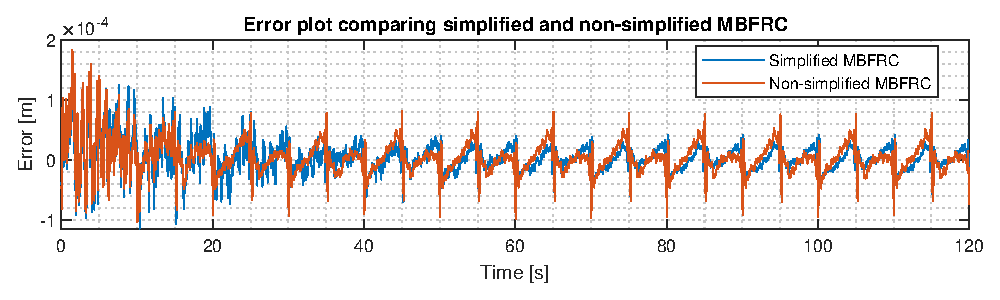
\includegraphics[width=0.8\linewidth]{./figures/nonSimple_MBFRC/comp_48freq_Err_2.eps}
    \caption{Comparison of error signal between simplified and non-simplified MBFRC with 48 attenuated frequencies}
    \label{fig: comp_48freq_Err_1}
\end{figure}

\subsection{Cascaded RC with MBFRC}
Since the MBFRC has proven to be very effective at quickly attenuating disturbances, the only disturbances that effectively remain are from the setpoint and its harmonics. Using a 'normal' RC controller in cascade with the MBFRC, as discussed in \autoref{ssec:cascadedRC}, should remove this last part of the error, without having to add frequencies for all of the maybe hundreds of harmonics that the setpoint brings. An experiment comparing simplified MBFRC with and without an added RC controller can be seen in \autoref{fig: withWithoutRC_comp_MBFRC_PSD_CAS_51}.
\begin{figure}
    \centering
    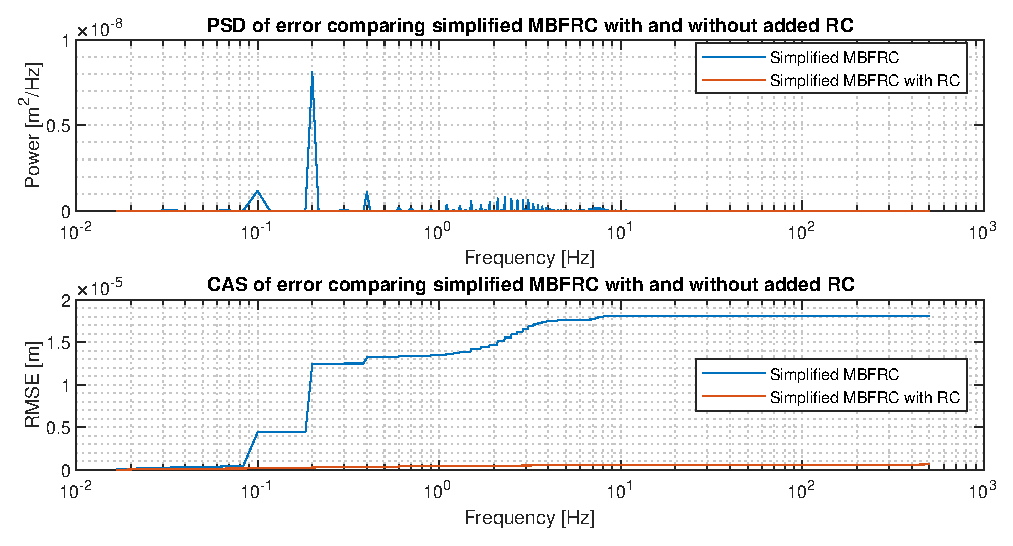
\includegraphics[width=0.9\linewidth]{figures/simple_RC_MBFRC/comp_48freq_PSD_CAS_2.eps}
    \caption{CPS and CAS of error signal using simplified MBFRC with and without an added RC controller in cascade}
    \label{fig: withWithoutRC_comp_MBFRC_PSD_CAS_51}
\end{figure}
Here it can be seen that adding the RC controller decreases the final error even more, from a RMS error of $1.813\cdot10^{-5}m$ to a value of $6.456\cdot10^{-7}m$, a factor 30 improvement.
\begin{figure}
    \centering
    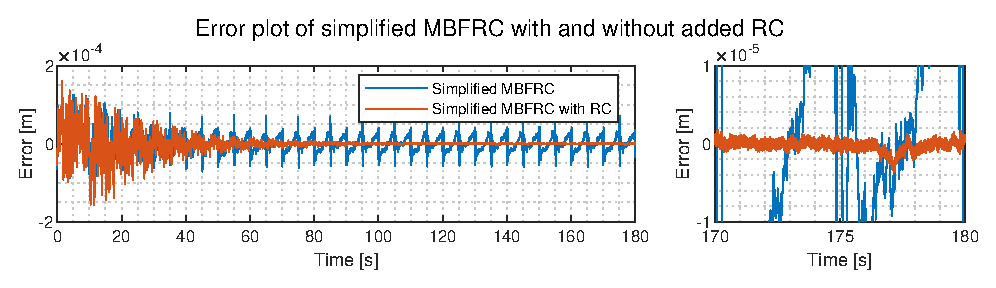
\includegraphics[width=1\linewidth]{figures/simple_RC_MBFRC/comp_48freq_Err_2.eps}
    \caption{Error signal using simplified MBFRC with and without an added RC controller in cascade (left), and a zoomed in version on the last $10$ seconds of the same error signal (right)}
    \label{fig: long_nonsimple_MBFRC_48_errsig}
\end{figure}

Using the cascaded RC with the non-simplified MBFRC as shown in \autoref{fig: simpleNonsimple_comp_nonsimple_MBFRC_Err_51} shows faster convergence than with simplified MBFRC, the resulting RMS error as gotten from the CAS in \autoref{fig: withWithoutRC_comp_nonsimple_MBFRC_PSD_CAS_51} seems to be slightly higher. However, the difference is roughly $6\cdot10^{-8}m$, which is in the region that the system heating up from electronics and friction might already have caused enough additional disturbances to make this difference. Therefore the difference is most likely not caused by the different algorithm but simply by a different time of measurement.

\begin{figure}
    \centering
    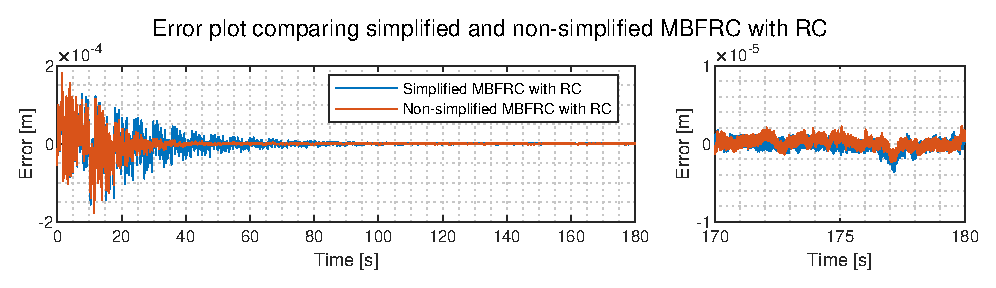
\includegraphics[width=1\linewidth]{figures/nonSimple_RC_MBFRC/compToSimple_48freq_Err_2.eps}
    \caption{Error signal comparing simplified to non-simplified MBFRC with an added RC controller in cascade}
    \label{fig: simpleNonsimple_comp_nonsimple_MBFRC_Err_51}
\end{figure}
\begin{figure}
    \centering
    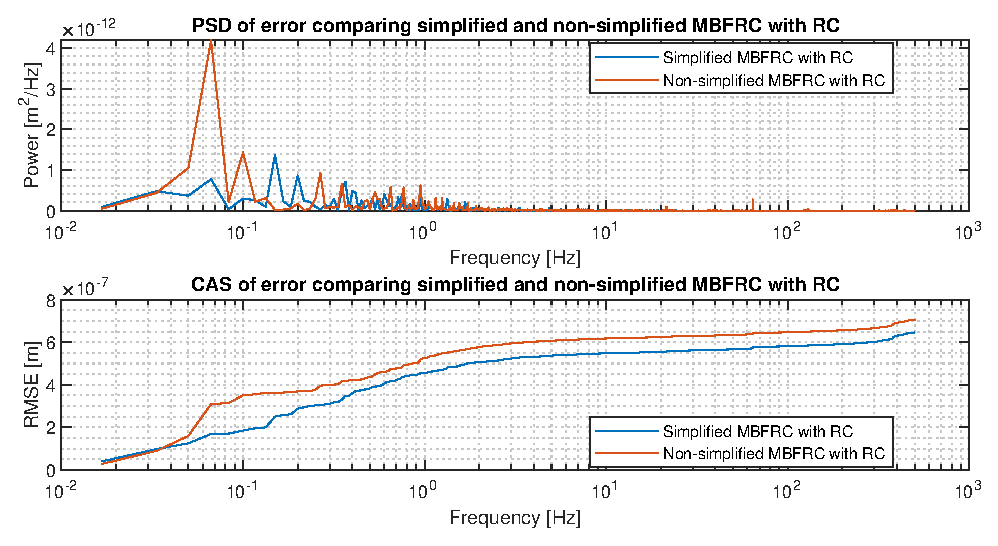
\includegraphics[width=1\linewidth]{figures/nonSimple_RC_MBFRC/compToSimple_48freq_PSD_CAS_2.eps}
    \caption{PSD and CAS of error signal using non-simplified MBFRC with and without an added RC controller in cascade (left), and a zoomed in version on the last $10$ seconds of the same error signal (right)}
    \label{fig: withWithoutRC_comp_nonsimple_MBFRC_PSD_CAS_51}
\end{figure}


The resulting final error is already very promising, however, further improvements were also attempted. The RC controller that is currently used is fairly conservative due to the used Q-filter, tuning this filter to take into account more frequencies is normally a good option to increase performance, but this does come at a cost of the robustness. Since the Q-filter was already tuned fairly conservatively, a Q-filter with a higher cut-off frequency was implemented and tested. The resulting CAS shown in \autoref{fig: Qfilt_comp_48freq_PSD_CAS_48} show that increasing this cut-off frequency does not improve the performance, the PSD is nearly identical for both versions of the Q-filter indicating their similarities as well. Taking a higher cut-off frequency actually introduces another very dominant frequency. This frequency appears to be much more dominant than before due to the waterbed effect. This will need to be explored in future research.
\begin{figure}
    \centering
    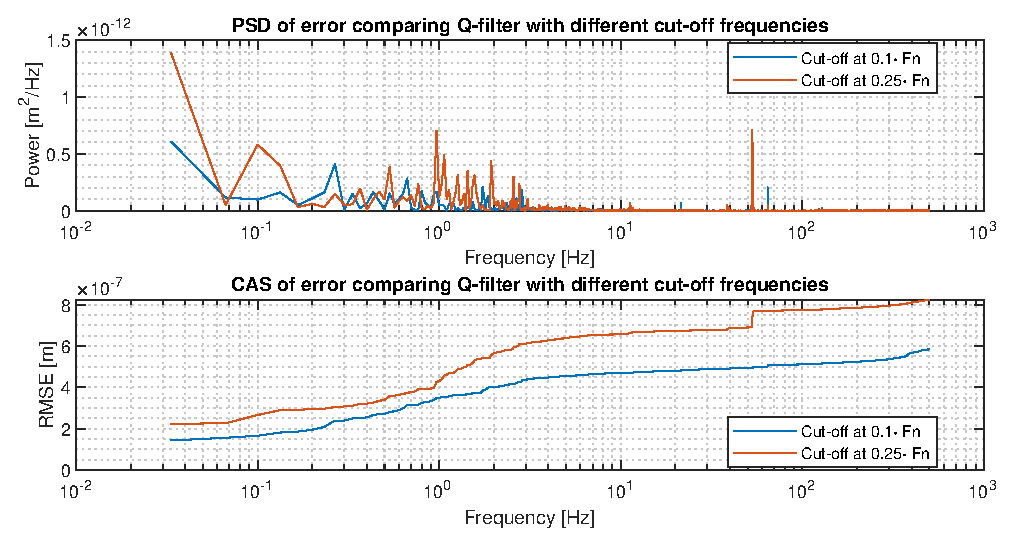
\includegraphics[width=1\linewidth]{figures/Q-filter/comp_48freq_PSD_CAS_2.eps}
    \caption{Error signal using non-simplified MBFRC RC controller, changing Q-filter cut-off}
    \label{fig: Qfilt_comp_48freq_PSD_CAS_48}
\end{figure}


\subsection{Parameter initialization}
To try and get faster convergence, the $\alpha_k$ values of a previous measurement were used as initial values for a next experiment. This should cause the $\alpha_k$'s to be closer to their final value, and thus decrease the total time needed to converge. The average of the last 3 setpoints from the previous experiment was used as the initial value of the simplified MBFRC's integrator. After the initialization the MBFRC was left to learn the same as without initialization. The resulting error plot comparing the performance with and without initialization can be seen in \autoref{fig: initTest_withWithoutInit_Err} together with how the values of the first $6\ \alpha_k$'s evolved over time.
\begin{figure}
    \centering
    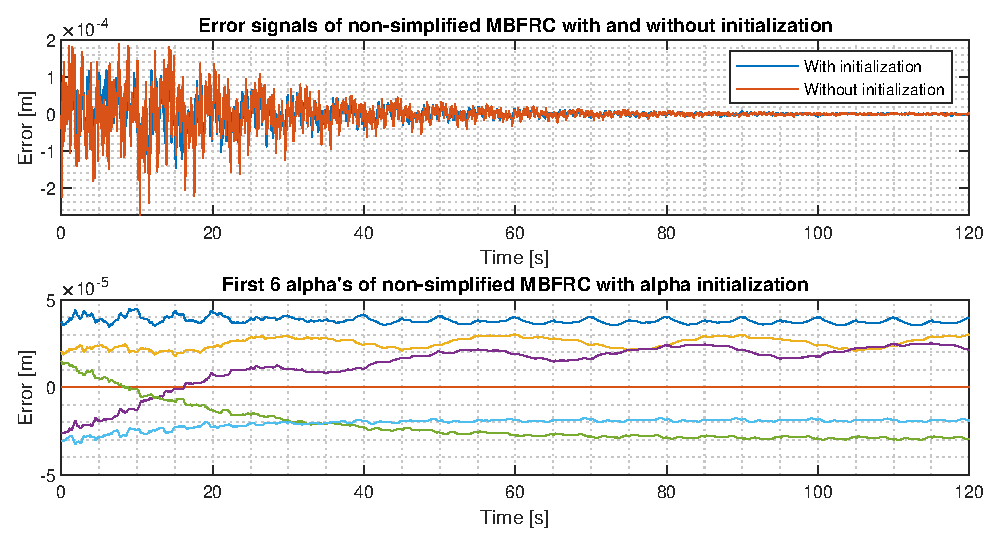
\includegraphics[width=1\linewidth]{figures/initTesting/comp_withWithoutInit_Err_2.eps}
    \caption{Error signal using simplified MBFRC with and without $\alpha$ initialization}
    \label{fig: initTest_withWithoutInit_Err}
\end{figure}
These figures show some unexpected behavior, as the $\alpha_k$'s do not seem to converge to the same values as in the previous experiment. This behavior makes the error even bigger in the beginning of the experiment, as the $\alpha_k$ values are further from their desired values than when initialized at $0$.

Additionally, the $\alpha_k$'s of a full back and forth motion of a previous experiment was applied inside the direct path of the integrator loop of the $\alpha_k$'s. Therefore applying this signal continuously for every back and forth motion of the Arizona, which might force the $\alpha_k$'s to converge to the same values as before.

However, this gave similar results to the average value initialization. Worsening the overal performance of the Arizona printer, while also increasing the complexity of the model. More research into the converge of the $\alpha_k$'s is needed before this application can be used to improve performance.

\subsection{Stability analysis implementation}
The stability analysis using non-linear optimization was implemented in MATLAB, using the script as found in \cite{github_2025_Learning_Control_2025}. Using this script, the maximum achievable $\phi$'s can be found. However, running this optimization script using the Arizona's model and controller always gives at least one eigenvalue with a larger absolute value than $1$. This indicates instability, the simulations and experiments give a different view as the system is clearly stabilizable, even with $48$ attenuated frequencies. This indicated that this method gives a very conservative approximation of when the system is stable, also indicating instability when in reality it is not. This difference likely comes from the fact that the model used for the MBFRC controller is an Linear Time Invariant estimate of the real MBFRC as it is normally not Time invariant. Other methods such as checking the Nyquist stability criteria might give less conservative solutions, this is however left to future research.

\section{Conclusion} \label{sec:Conclusion}
%What did your work reveal? What does this mean for the reader? Make sure it connects with your introduction. Additionally, add recommendation for future work/research.
This research successfully demonstrated the effectiveness of MBFRC in suppressing multi frequency disturbances in a complex industrial system. Through simulation and experimental verification on the Arizona printer, both simplified and non-simplified MBFRC significantly improved disturbance rejection performance compared to conventional control methods. In summary, simplified MBFRC effectively provided similar disturbance reduction as the non-simplified MBFRC with a more straightforward implementation, while non-simplified MBFRC notably enhanced convergence speed. In addition to this, promising results were shown by putting a traditional RC controller in a cascaded manner with MBFRC. Though this requires additional research for stability before it can be used in industrial settings.

These findings emphasize the practicality that MBFRC techniques can offer for industrial systems, particularly in managing disturbances where traditional methods fall short. The modular nature of the attenuated frequencies highlights its suitability for real world applications, while also meeting an increasingly important industrial criterion: performance.

Future work should explore further optimization of MBFRC parameters, implementing techniques to reduce manual tuning and give less conservative stability guarantees. Investigating the effect of the robustness filter $Q$ in the cascaded RC controller could also broaden the capability and effectiveness of MBFRC in varied industrial systems. Initialization of parameters according to a previously found optimum could be a promising field to improve a system's convergence speed while leaving performance unaltered. More research into MBFRC's parameters and their respective converged values is needed for this technique to be applicable in industry.

\bibliographystyle{IEEEtran}  % or another style like plain, alpha, etc.
\bibliography{references}     % references.bib is your BibTeX file

\appendices
\section{Introductory figures}
The disturbance signal is artificially inserted into the system, with this disturbance signal already known. The disturbance signal's PSD can be seen in \autoref{fig: PSD_disturbance_real}, clearly showing which frequencies the disturbance consists of. The reference signal used for the simulations and experiments is also already defined, with it being shown in \autoref{fig:yref}. As can be seen, the Arizona printer should follow a back and forth motion with an amplitude of $2m$, with one reference consisting of 3 back and forth motions. 
\begin{figure}[!b]
    \centering
    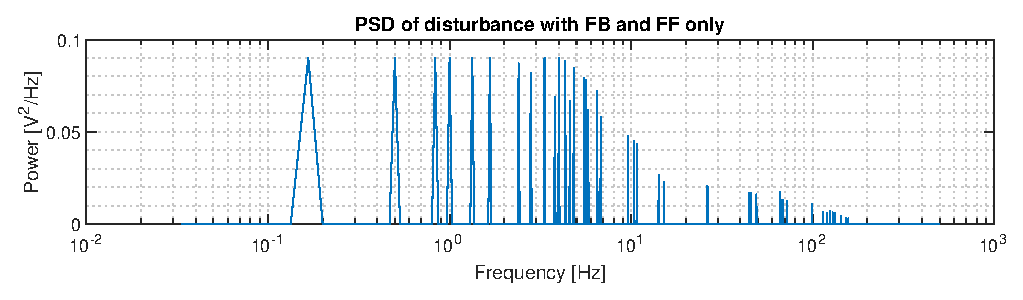
\includegraphics[width=1\linewidth]{figures/General/disturbancePower_real_2.eps}
    \caption{Power Spectral Density of disturbance signal applied to the system}
    \label{fig: PSD_disturbance_real}
\end{figure}
\begin{figure}
    \centering
    \includegraphics[width=1\linewidth]{figures/General/Ref.eps}
    \caption{Reference signal applied to the y-axis of the Arizona printer.}
    \label{fig:yref}
\end{figure}

\section{Simuations with simplified MBFRC}\label{app:SimSim}
Due to space limitations some more results of simulations are shown here in the appendix. They will have some short explanation as well. \autoref{fig:sim48simp} shows the best performing simulation for simplified MBFRC where 48 frequencies are attenuated. Results about this are discussed in \autoref{sssec: SimplifiedMBFRC_Simulation}. \autoref{fig:fftSimp48} shows a PSD and CAS of the simulation with 48 frequencies. It shows that all the frequencies are still present but attenuated to a power of at most \(6*10^-7\). \autoref{fig:SimSimp20} shows the simulation results of attenuating 20 frequencies with a $\phi = 0.001$. This shows that the convergence is much faster but the achieved L2 norm is significantly worse compared to attenuating 48 frequencies. \autoref{fig:fftSimp20} shows the PSD and CAS of the simulation where 20 frequencies are attenuated. This shows that the 20 attenuated frequencies are so small that they can not be seen compared to the frequencies that are not attenuated. \autoref{fig:SimSimp10} shows that for 10 frequencies the convergence is even faster but the remaining error is much greater, this was reached with $\phi =0.002$. \autoref{fig:fftSimp10} shows the PSD and CAS for 10 attenuated frequencies, it is clear that a lot more frequencies are still present in the system.
\begin{figure}
    \centering
    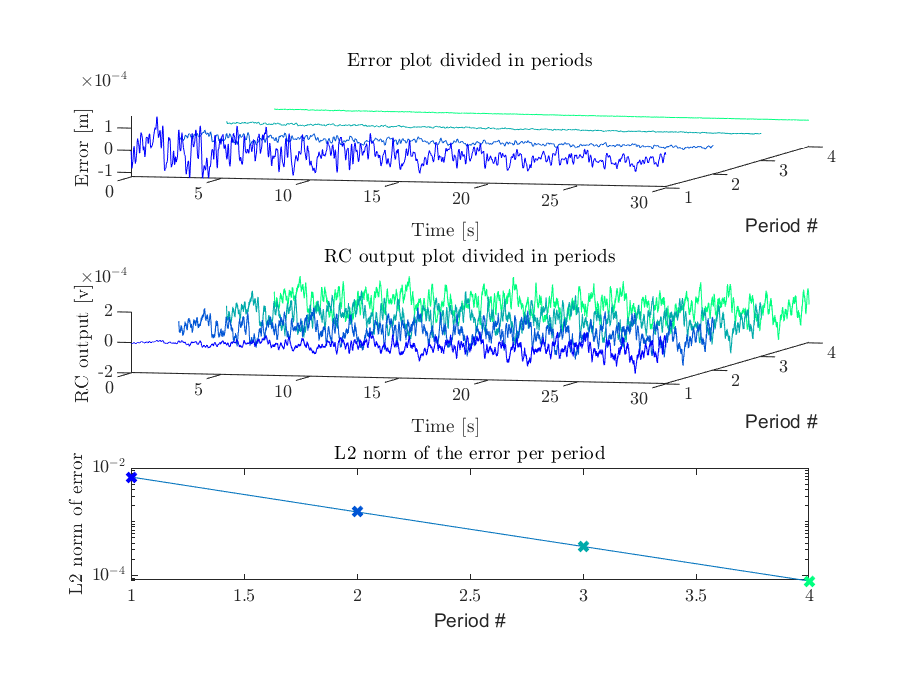
\includegraphics[width=1\linewidth]{figures/simple_MBFRC/SimulationSimp48.eps}
    \caption{Plot showing the best results with MBFRC while attenuating 48 frequencies.}
    \label{fig:sim48simp}
\end{figure}
\begin{figure}
    \centering
    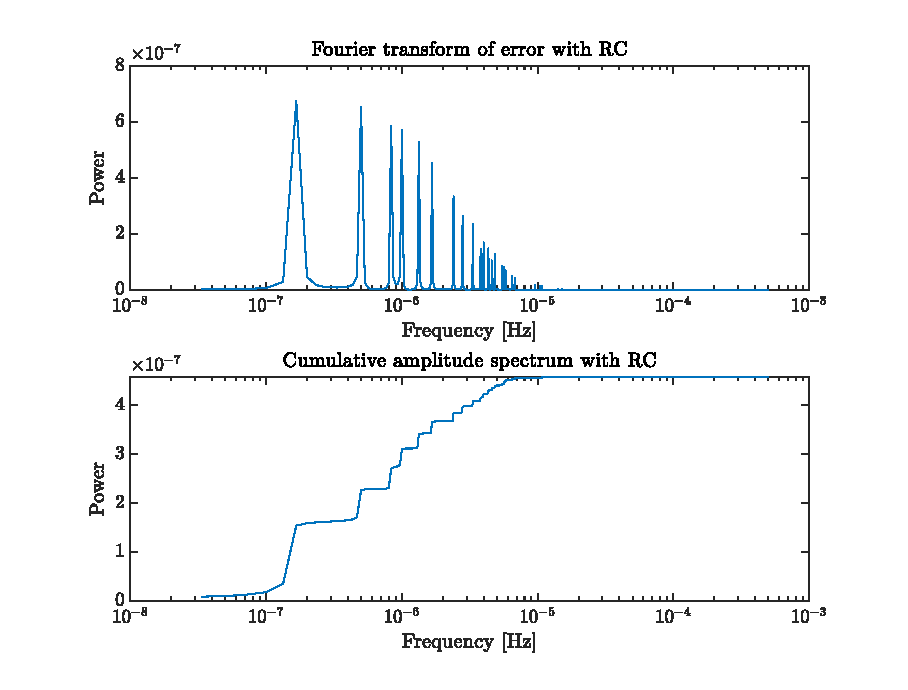
\includegraphics[width=1\linewidth]{figures/simple_MBFRC/FourierSimp48.eps}
    \caption{PSD and CAS of simplified MBFRC simulation with 48 attenuated frequencies.}
    \label{fig:fftSimp48}
\end{figure}
\begin{figure}
    \centering
    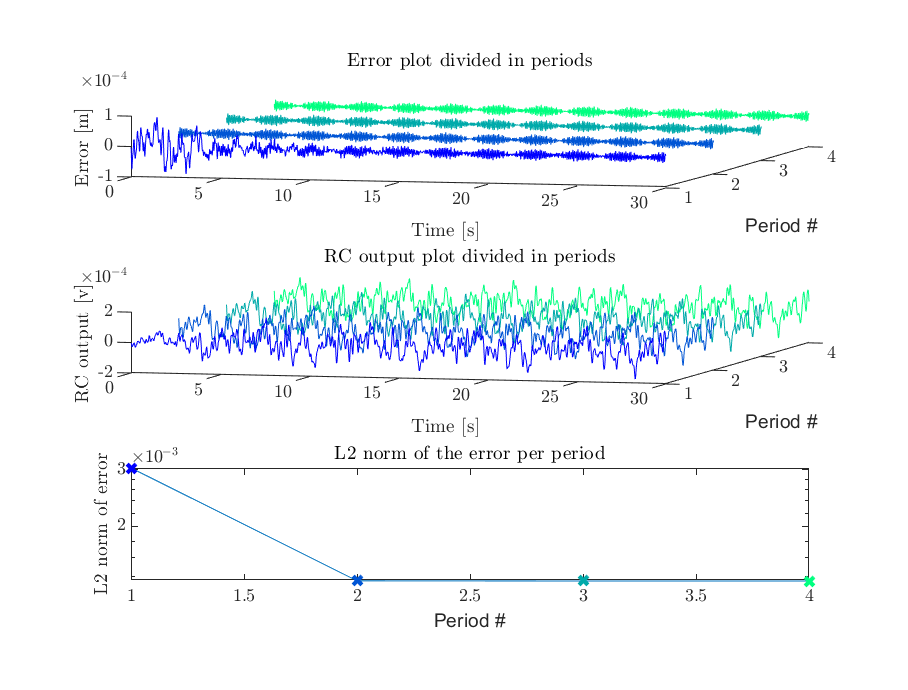
\includegraphics[width=1\linewidth]{figures/simple_MBFRC/SimulationSimp20.eps}
    \caption{Simulation results of attenuating 20 frequencies using simplified MBFRC.}
    \label{fig:SimSimp20}
\end{figure}
\begin{figure}
    \centering
    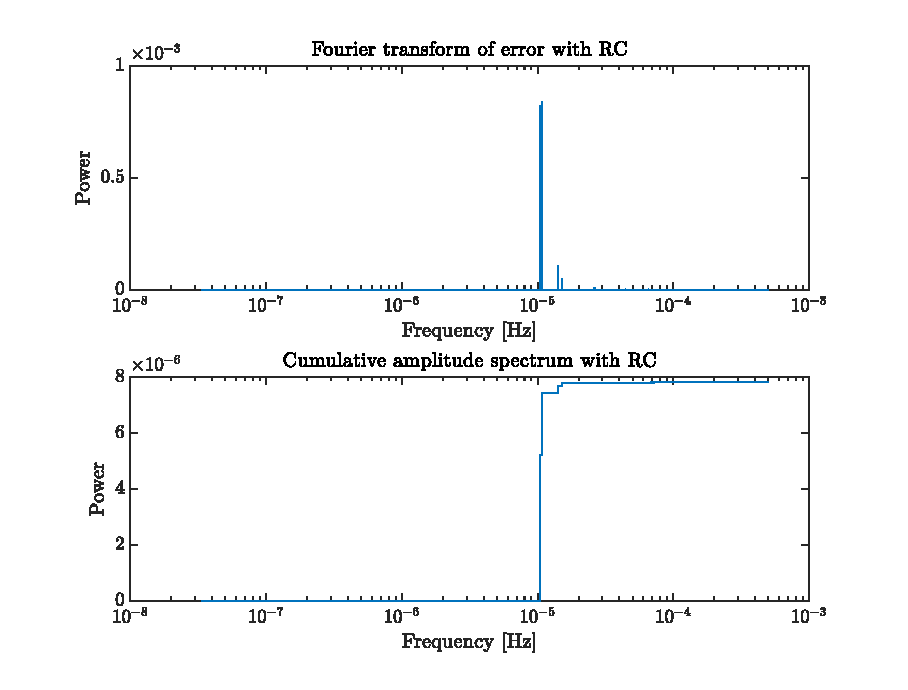
\includegraphics[width=1\linewidth]{figures/simple_MBFRC/FourierSimp20.eps}
    \caption{PSD and CAS of simplified MBFRC simulation with 20 attenuated frequencies.}
    \label{fig:fftSimp20}
\end{figure}
\begin{figure}
    \centering
    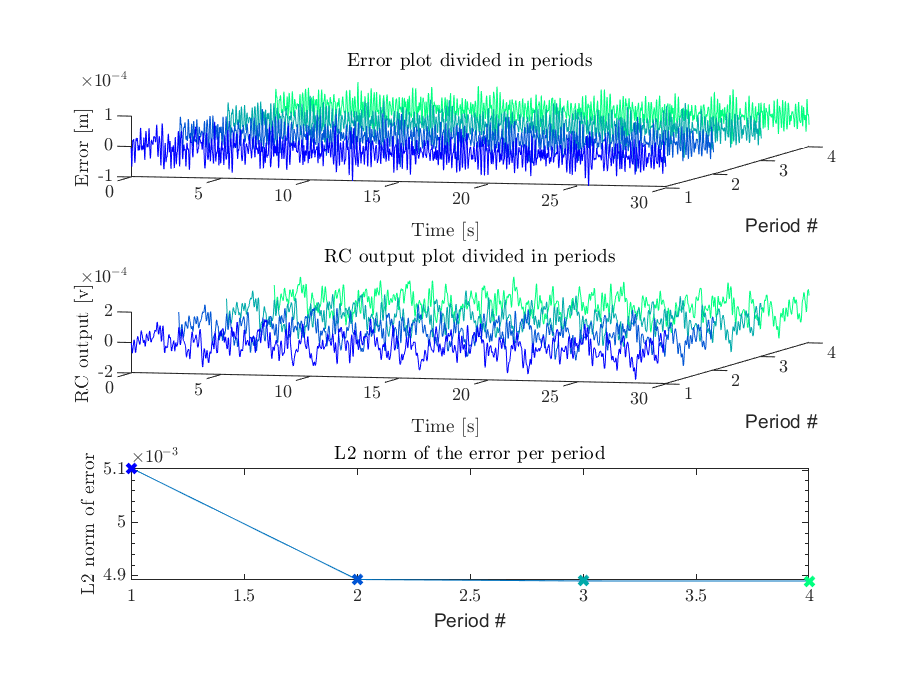
\includegraphics[width=1\linewidth]{figures/simple_MBFRC/SimulationSimp10.eps}
    \caption{Simulation results of attenuating 10 frequencies using simplified MBFRC.}
    \label{fig:SimSimp10}
\end{figure}
\begin{figure}
    \centering
    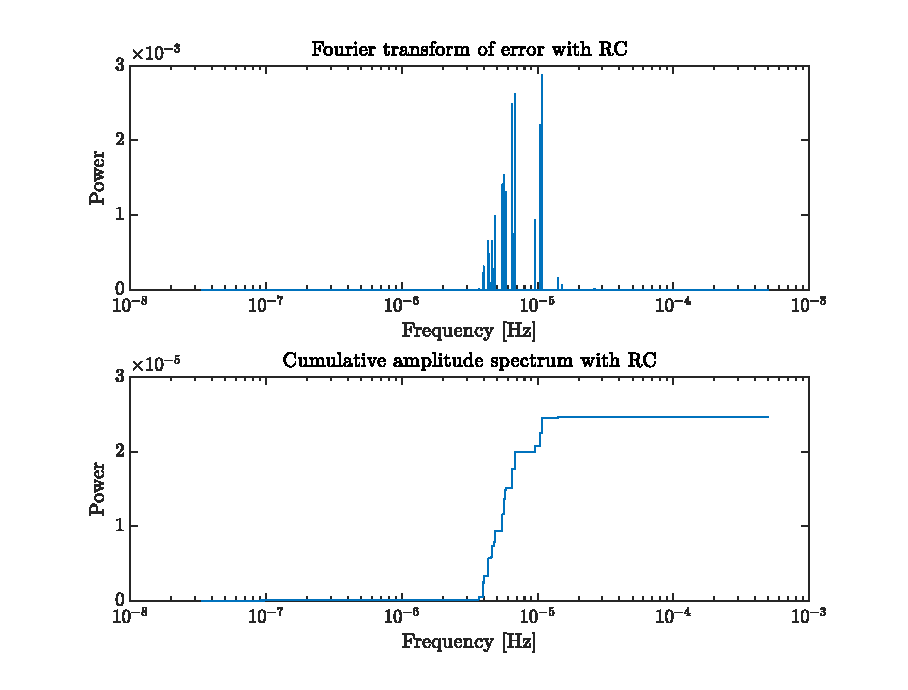
\includegraphics[width=1\linewidth]{figures/simple_MBFRC/FourierSimp10.eps}
    \caption{PSD and CAS of simplified MBFRC simulation with 20 attenuated frequencies.}
    \label{fig:fftSimp10}
\end{figure}
\section{Simulations with non-simplified MBFRC}\label{app:nonSimSim}
Due to space limitations some more results of simulations are shown here in the appendix. \autoref{fig:nonSimpSim48} shows the best simulation result where 48 frequencies are being attenuated. The specifics are described in \autoref{sssec: NonSimplifiedMBFRC_Simulation} \autoref{fig:fftNonSimp48} shows that the values have becomes so low that even the disturbance frequencies are not showing up anymore. The remaining peak is just some mathematical error in Matlab as there is no disturbance at that frequency. \autoref{fig:SimNonSimp20} shows that the error is being rejected even faster than before but a lot of error remains such that the L2 norm is still relatively high. \autoref{fig:fftNonSimp20} shows that the 20 frequencies are removed but the higher frequencies still remain completely untouched. \autoref{fig:SimSimp10} shows that the 10 frequencies are being rejected quickly but it is not enough to make a big impact on the error of the system. \autoref{fig:fftNonSimp10} shows that the 10 frequencies are being atttenuated but still a lot of power remains in the other frequencies.

\begin{figure}
    \centering
    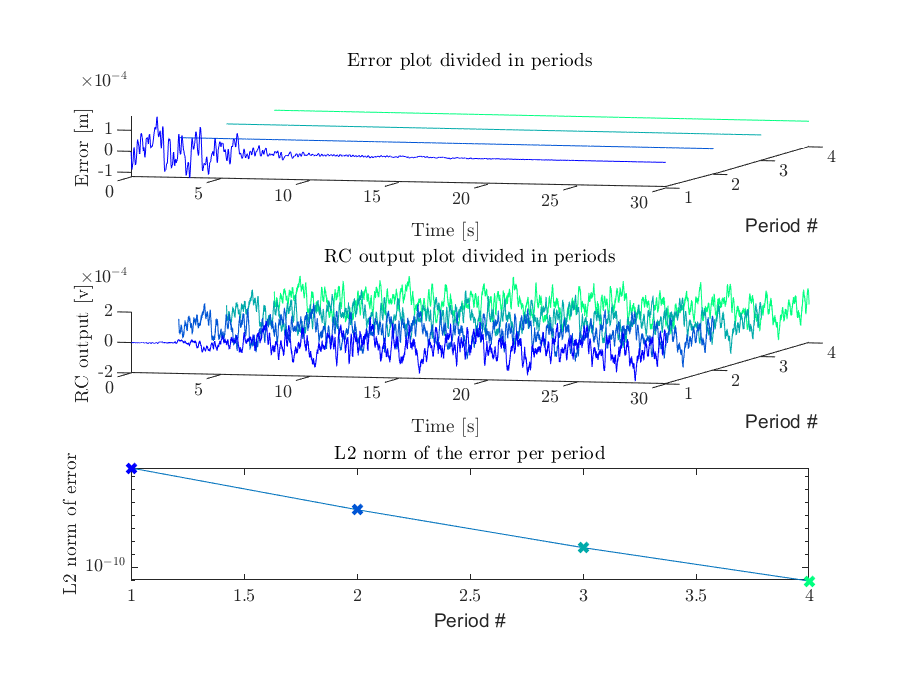
\includegraphics[width=1\linewidth]{figures/nonSimple_RC_MBFRC/SimulationNonSimp48.eps}
    \caption{Simulation showing the results of attenuating 48 frequencies using non-simplified MBFRC.}
    \label{fig:nonSimpSim48}
\end{figure}
\begin{figure}
    \centering
    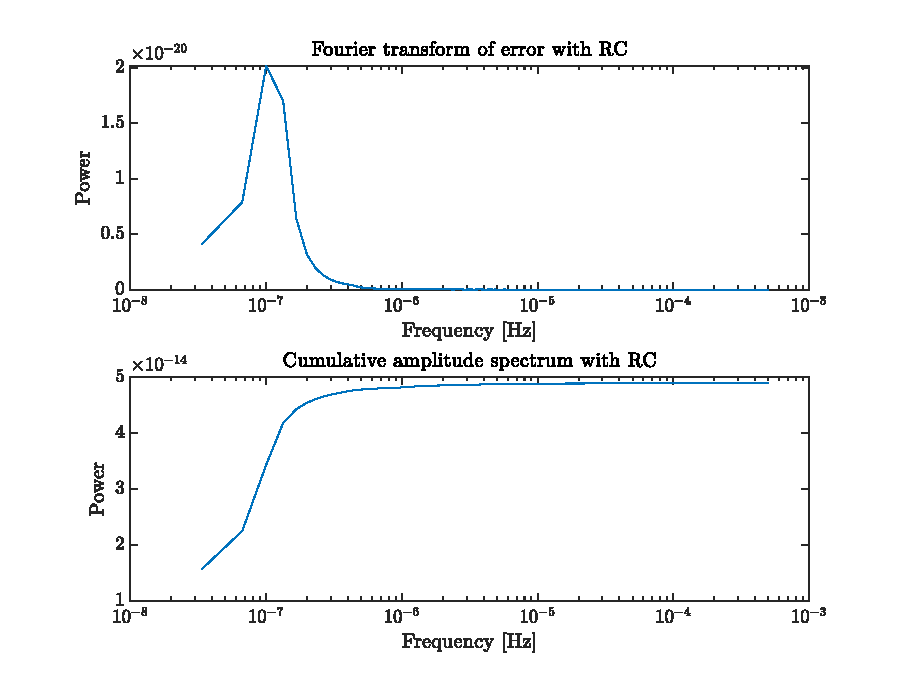
\includegraphics[width=1\linewidth]{figures/nonSimple_RC_MBFRC/FourierNonSimp48.eps}
    \caption{PSD and CAS of non-simplified MBFRC simulation with 48 attenuated frequencies.}
    \label{fig:fftNonSimp48}
\end{figure}
\begin{figure}
    \centering
    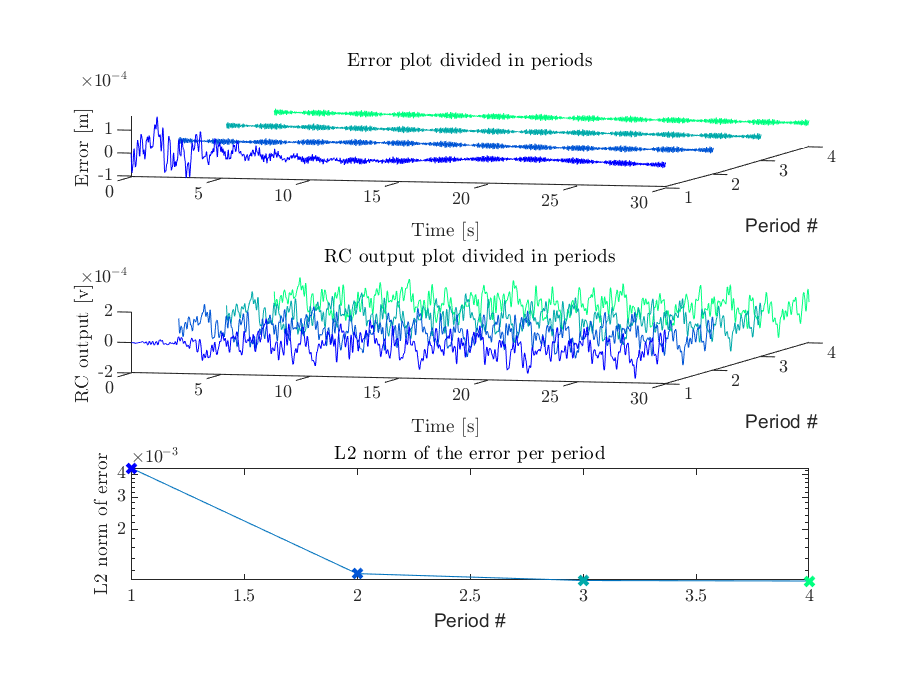
\includegraphics[width=1\linewidth]{figures/nonSimple_RC_MBFRC/SimulationNonSimp20.eps}
    \caption{Simulation results of attenuating 20 frequencies using non-simplified MBFRC.}
    \label{fig:SimNonSimp20}
\end{figure}
\begin{figure}
    \centering
    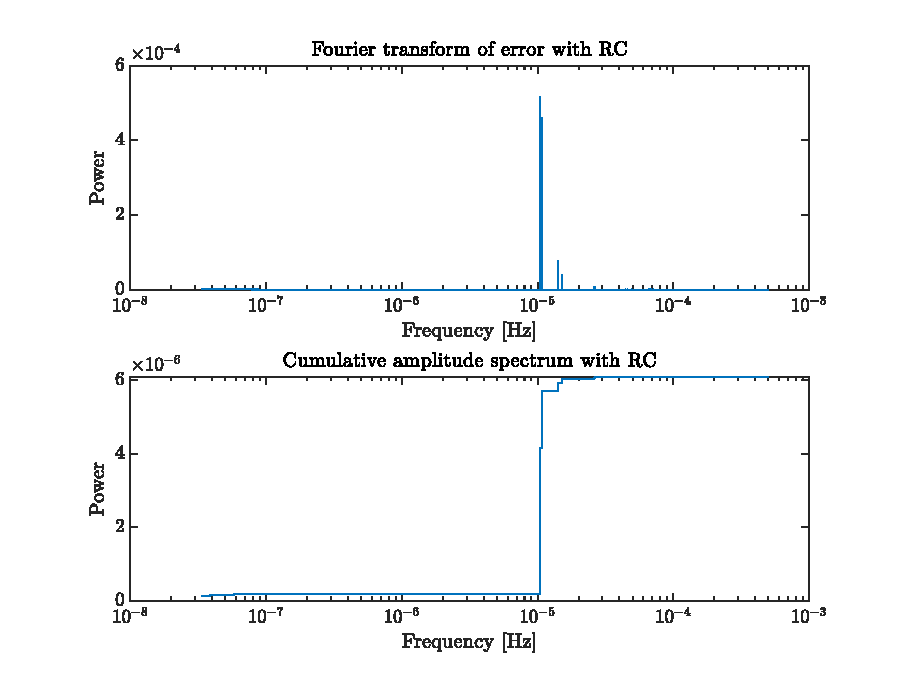
\includegraphics[width=1\linewidth]{figures/nonSimple_RC_MBFRC/FourierNonSimp20.eps}
    \caption{PSD and CAS of non-simplified MBFRC simulation with 20 attenuated frequencies.}
    \label{fig:fftNonSimp20}
\end{figure}
\begin{figure}
    \centering
    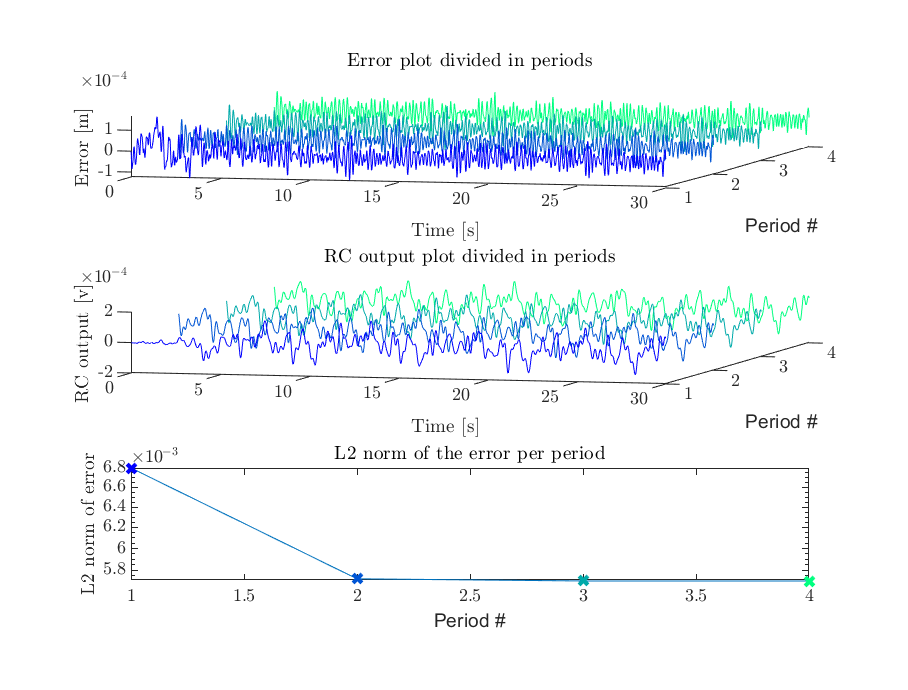
\includegraphics[width=1\linewidth]{figures/nonSimple_RC_MBFRC/SimulationNonSimp10.eps}
    \caption{Simulation results of attenuating 10 frequencies using non-simplified MBFRC.}
    \label{fig:SimNonSimp10}
\end{figure}
\begin{figure}
    \centering
    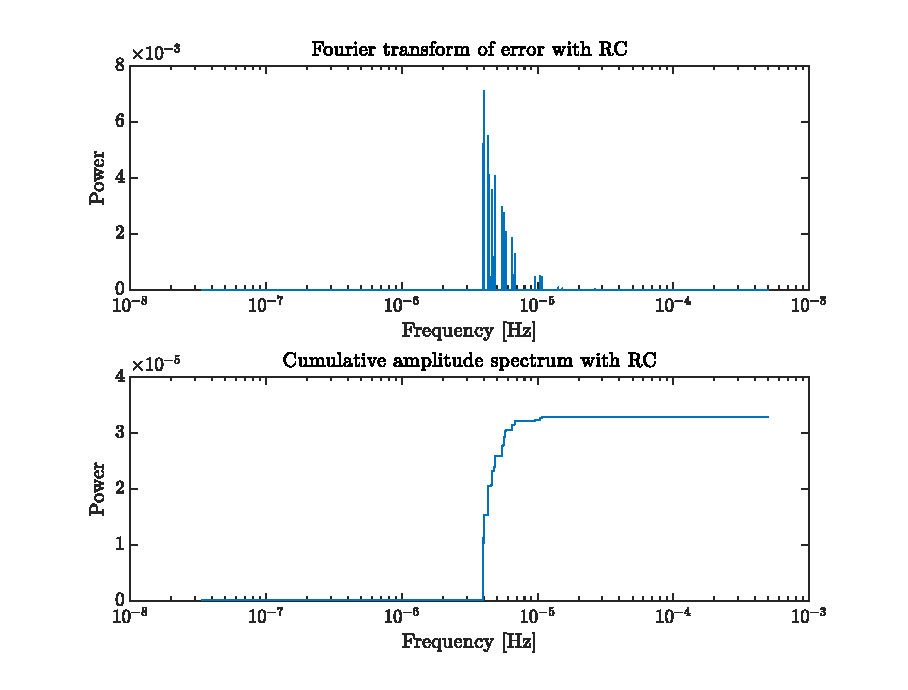
\includegraphics[width=1\linewidth]{figures/nonSimple_RC_MBFRC/FourierNonSimp10.eps}
    \caption{PSD and CAS of non-simplified MBFRC simulation with 10 attenuated frequencies.}
    \label{fig:fftNonSimp10}
\end{figure}
\section{Simulations with cascaded RC and MBFRC}\label{app:simCasc}
The best performing simulation for the cascaded RC structure is shown in \autoref{fig:cascNonSimp} where the results are discussed further in \autoref{sssec:CascadedSim}.

\begin{figure}
    \centering
    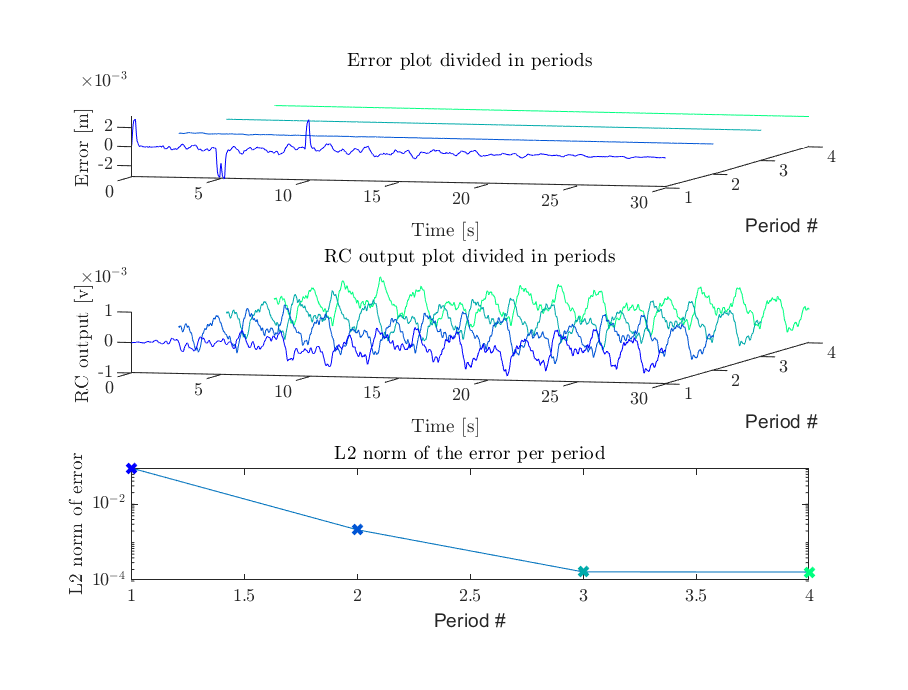
\includegraphics[width=1\linewidth]{figures/nonSimple_RC_MBFRC/SimCascNon.eps}
    \caption{Simulation results of the cascaded design with non-simplified MBFRC}
    \label{fig:cascNonSimp}
\end{figure}


% \section{Matlab code} \label{app:code}
% Any relevant pieces of Matlab code may be added in the appendices. We have provided some code to help you export an open figure from Matlab in PDF format. The use of either PDF or EPS format for your figures is recommended. 
% Before creating a figure, set the interpreter to \LaTeX. 

% \lstinputlisting{./matlab/fig_settings.m}

% Then, set the width of the figure equal to that of the columns in this template and save the figure in PDF format.

% \lstinputlisting{./matlab/exp_pdf.m}

% % you can choose not to have a title for an appendix
% % if you want by leaving the argument blank
% \section{Appendix subtitle goes here.}
% Appendix B text goes here.



% references section

% can use a bibliography generated by BibTeX as a .bbl file
% BibTeX documentation can be easily obtained at:
% http://mirror.ctan.org/biblio/bibtex/contrib/doc/
% The IEEEtran BibTeX style support page is at:
% http://www.michaelshell.org/tex/ieeetran/bibtex/
%\bibliographystyle{IEEEtran}
% argument is your BibTeX string definitions and bibliography database(s)
%\bibliography{IEEEabrv,../bib/paper}
%
% <OR> manually copy in the resultant .bbl file
% set second argument of \begin to the number of references
% (used to reserve space for the reference number labels box)





% that's all folks
\end{document}